
%(BEGIN_QUESTION)
% Copyright 2009, Tony R. Kuphaldt, released under the Creative Commons Attribution License (v 1.0)
% This means you may do almost anything with this work of mine, so long as you give me proper credit

Read and outline the ``Capacitive'' section of the ``Continuous Level Measurement'' chapter in your {\it Lessons In Industrial Instrumentation} textbook.  Note the page numbers where important illustrations, photographs, equations, tables, and other relevant details are found.  Prepare to thoughtfully discuss with your instructor and classmates the concepts and examples explored in this reading.

\underbar{file i03964}
%(END_QUESTION)





%(BEGIN_ANSWER)


%(END_ANSWER)





%(BEGIN_NOTES)

If a rod is inserted into a metal vessel, capacitance between that rod and the vessel will increase as level increases:

$$C = {\epsilon A \over d}$$

Conductive liquids use a plastic-coated rod, with the plastic being the dielectric and the conductive liquid being an extension of the conductive tank wall.

\vskip 10pt

Non-conductive liquids use a bare metal rod, with the liquid itself being the dielectric.  Here, process liquid dielectric permittivity is an important factor in measurement accuacy.  Sometimes capacitive level instruments use a constantly-immersed {\it compensation probe} to continually measure the permittivity of the liquid, in order to automatically compensate for changes in liquid permittivity.

\vskip 10pt

Solids are also measurable using this technology (non-conductive), although variations in moisture content may radically affect permittivity.

\vskip 10pt

Stray capacitance in probe cables and other components is a significant source of measurement error in these systems.











\vskip 20pt \vbox{\hrule \hbox{\strut \vrule{} {\bf Suggestions for Socratic discussion} \vrule} \hrule}

\begin{itemize}
\item{} {\bf In what ways may a capacitive level instrument be ``fooled'' to report a false level measurement?}
\item{} Identify a factor other than liquid $\epsilon$ that can cause a non-capacitive level transmitter to register a falsely positive (too high) product height.
\item{} Identify a factor other than liquid $\epsilon$ that can cause a non-capacitive level transmitter to register a falsely negative (too low) product height.
\item{} If liquid $\epsilon$ increases in a non-conductive capacitance level application, what is the effect on level measurement?
\item{} If liquid $\epsilon$ decreases in a non-conductive capacitance level application, what is the effect on level measurement?
\item{} If the liquid in a non-conductive capacitance level application suddenly becomes conductive, what is the effect on level measurement?
\item{} Apply the concept of a {\it compensation probe} used on some capacitive level instruments to a different level-sensing technology, identifying not only what would be compensated for, but also what the compensating component(s) would be.
\end{itemize}















\vfil \eject

\noindent
{\bf Prep Quiz:}

Capacitive level sensors come in two basic varieties: those with ``coated'' probe wires and those with bare probe wires.  Identify the process liquid characteristic necessitating one type of probe versus the other:

\begin{itemize}
\item{} Density
\vskip 5pt 
\item{} Conductivity
\vskip 5pt 
\item{} Temperature
\vskip 5pt 
\item{} Viscosity
\vskip 5pt 
\item{} Color
\vskip 5pt 
\item{} Turbidity
\end{itemize}


\vfil \eject

\noindent
{\bf Summary Quiz:}

Determine what will happen in this AC circuit as the liquid level inside the tank rises (assuming the liquid is a good insulator, meaning it has a high permittivity value):

$$\includegraphics[width=15.5cm]{i03964x01.eps}$$

\begin{itemize}
\item{} Voltage across the source will increase 
\vskip 5pt 
\item{} Current in the circuit will decrease
\vskip 5pt 
\item{} The liquid will begin to cool down rapidly
\vskip 5pt 
\item{} Voltage across the source will decrease
\vskip 5pt 
\item{} The circuit will begin to resonate
\vskip 5pt 
\item{} Voltage drop across the resistor will increase
\end{itemize}

%INDEX% Reading assignment: Lessons In Industrial Instrumentation, Continuous Level Measurement (capacitance)

%(END_NOTES)


